% ****** Start of file apssamp.tex ******
%
%   This file is part of the APS files in the REVTeX 4.2 distribution.
%   Version 4.2a of REVTeX, December 2014
%
%   Copyright (c) 2014 The American Physical Society.
%
%   See the REVTeX 4 README file for restrictions and more information.
%
% TeX'ing this file requires that you have AMS-LaTeX 2.0 installed
% as well as the rest of the prerequisites for REVTeX 4.2
%
% See the REVTeX 4 README file
% It also requires running BibTeX. The commands are as follows:
%
%  1)  latex apssamp.tex
%  2)  bibtex apssamp
%  3)  latex apssamp.tex
%  4)  latex apssamp.tex
%
\documentclass[%
 reprint,
%superscriptaddress,
%groupedaddress,
%unsortedaddress,
%runinaddress,
%frontmatterverbose, 
%preprint,
%preprintnumbers,
%nofootinbib,
%nobibnotes,
%bibnotes,
 amsmath,amssymb,
 aps,
%pra,
%prb,
%rmp,
%prstab,
%prstper,
%floatfix,
]{revtex4-2}

\usepackage{hyperref}
\usepackage{mathtools}
\usepackage{textgreek}
\usepackage[nolist]{acronym}
\usepackage{braket}
\usepackage{amssymb}
\usepackage{amsmath}
\usepackage{graphicx}% Include figure files
\usepackage{dcolumn}% Align table columns on decimal point
\usepackage{bm}% bold math
%\usepackage{hyperref}% add hypertext capabilities
%\usepackage[mathlines]{lineno}% Enable numbering of text and display math
%\linenumbers\relax % Commence numbering lines

%\usepackage[showframe,%Uncomment any one of the following lines to test 
%%scale=0.7, marginratio={1:1, 2:3}, ignoreall,% default settings
%%text={7in,10in},centering,
%%margin=1.5in,
%%total={6.5in,8.75in}, top=1.2in, left=0.9in, includefoot,
%%height=10in,a5paper,hmargin={3cm,0.8in},
%]{geometry}

\begin{document}

\preprint{APS/123-QED}

\title{Eigenvector continuation mini-review}% Force line breaks with \\

\author{Kyle Beyer}
\affiliation{
  University of Michigan \\
  Department of Nuclear Engineering and Radiological Science
}%




\date{\today}% It is always \today, today,
             %  but any date may be explicitly specified

\begin{abstract}
  This brief article summarizes several key aspects of eigenvector continuation, a recent approximation technique in quantum mechanics. Eigenvector continuation projects a Hamiltonian which smoothly varies with a parameter, onto a training subspace spanned by high-quality solutions of eigenvectors for a set of realizations of that parameter. Thus, it allows for computationally efficient interpolation and extrapolation of eigenvectors to parameter values not in the
  training set. Conceptually, this is successful because, if a bounded linear operator acting on a Hilbert space varies smoothly with a parameter, the trajectories of its eigenvectors and eigenvalues will lie in a smooth manifold of much lower dimension than the eigenspace of the operator. 

  The focus of the review is to briefly survey the literature for applications of this method, and provide a pedagogical introduction. It is formally derived, motivated with a conceptual comparison to a perturbative approach, and some limitations and convergence properties are explored. For the sake of brevity, complicating features like
  excited states, degeneracy, larger than 1 dimensional parameter spaces, and choice of training subspace are are largely ignored, but have been explored in the literature.
\end{abstract}

%\keywords{Suggested keywords}%Use showkeys class option if keyword
                              %display desired
\maketitle


%\tableofcontents

\begin{acronym}
  \acro{CEFT}[$\chi$EFT]{Chiral effective field theory}
  \acro{EC}{Eigenvector continuation}
  \acro{LEC}{Low Energy Constants}
  \acro{UQ}{Uncertainty Quantification}
\end{acronym}

\section{\label{sec:mot}Introduction and Motivation}
The eigenvalue problem is ubiquitous in science and engineering, as the vast majority of systems can be modeled as linear. In many cases, these models are not purely ab-initio, and contain degrees of freedom constrained by experimental observations. Often, computational tractability imposes a practical limitations on the success of marrying theory to experiment; or phenomenology, in a broad sense.
Ideally, one could use Bayesian inference to determine optimal free parameters in a physical theory to match experimental observations with quantified uncertainties that include prior assumptions, but the computational expense of repeated evaluation of the likelihood ratio makes this technique unsuitable for problems at the forefront of computational physics \cite{king2019direct,box2011bayesian}. 

In quantum mechanics, examples of such problems include strongly-coupled many-body
systems. \ac{CEFT} calculations of nuclear structure, and ultra-cold gasses, are two such examples. In fact, it is often only tractable, or even possible, to conduct simulations with certain simplifying assumptions. One is then forced to extrapolate from the solvable regime to the regime of interest for experimental comparison. 

Recently, the Rayleigh-Ritz method \cite{jia2001analysis,knyazev1997new,jia1999convergence,saad2000introduction} has enjoyed a renaissance in applications to such problems in quantum mechanics, under the name
\ac{EC}. Conceptually, this technique relies on the fact that trajectories of eigenvalues and eigenvectors dependent on some parameter in their associated operator lie on a manifold of much lower dimension than the full eigenspace of the operator, as long as the operator varies smoothly in the parameter. This technique was initially formulated and applied in 2018 to extending \ac{CEFT} to the non-perturbative regime \cite{frame2018eigenvector,frame2019ab}.

In subsequent years, \ac{EC} has enjoyed applications in two different modalities: to construct emulators for a parameter dependent eigenvalue solver for efficient Bayesian inference on a model parameter space, as well as to extrapolate eigenkets and eigenvalues from the perturbative regime to the non-perturbative regime. 

The former of these two has seen applications towards doing \ac{UQ} of potential parameters in mean-field (Hartree-Fock) nuclear reaction theory \cite{drischler2021toward,furnstahl2020efficient,konig2020eigenvector}, as well as in \ac{UQ} and sensitivity analysis of \ac{LEC}s in \ac{CEFT} nuclear structure calculations \cite{ekstrom2019global}.

The latter has seen applications in atomic systems \cite{demol2020improved}, strongly interacting cold systems \cite{eklind2021eigenvector}, and incorporated into many-body perturbation theory \cite{demol2021bogoliubov}. Reference \cite{eklind2021eigenvector} provides a nice derivation of the method, and presents techniques for optimal choice of training subspace (which are beyond the scope of the current work).

This article is organized as follows. Section \ref{sec:der} derives the method. Section \ref{sec:comp} compares \ac{EC} to perturbation theory for a simple theoretical case, as well as in practice. Section \ref{sec:lim} very briefly summarizes the convergence properties and limitations of \ac{EC}, and Section \ref{sec:appl} highlights some interesting results from the literature cited above.


\section{\label{sec:der}Formal Derivation}

Consider a bounded linear operator $H(\lambda) : \mathcal{H}(\lambda) \rightarrow \mathcal{H}(\lambda)$, acting on a Hilbert space $\mathcal{H}(\lambda)$ (or more commonly a subset of a Hilbert space) equipped with some inner product $\Braket{\cdot|\cdot}$, and smoothly varying with some parameter $\lambda$. We denote the Hilbert space $\mathcal{H}(\lambda)$ to make explicit that the space itself also varies with $\lambda$, in the sense that, for two distinct realizations of $\lambda$, the
corresponding Hilbert spaces may not be isomorphic, and, subsequently, the span of one may be incomplete to construct a vector in the other. We introduce the superset of Hilbert spaces $H_S \vcentcolon= \cup_{\lambda \in \mathbb{D}}  \mathcal{H}(\lambda)$.

We allow $\lambda$ to run over some domain $\mathbb{D}$, e.g. a subset of $\mathbb{R}$.  We may construct an eigenvalue equation for a realization of our operator:

\begin{equation}
  \left( H(\lambda) - E(\lambda)  \right) \ket{\phi(\lambda)} = 0.
\end{equation}

In quantum mechanics, we may associate $H(\lambda)$ with the Hamiltonian of a system that depends on $\lambda$. For instance, $\lambda$ could be the strength of a magnetic field applied to an atom, the coupling between particles in a many-body system, the depth of a potential well, etc. In more practical cases, it could be (semi-)phenomenological parameters in a model, that are constrained or fit by experiment. For example, these could be the optical model potential parameters, or \ac{CEFT}
\ac{LEC}s.

In the case that $H$ is a Hamiltonian operator, the minimal eigenvalue $E(\lambda)$ can be associated with the ground state energy
of the system, and, likewise, the corresponding eigenvector with the ground state. In this case, our inner product is of the usual Hermitian type; $\Braket{\phi_1|\phi_1} \in \mathbb{R}$.

One desires to approximate the realization of the eigenvalue and eigenket for a given target parameter, $\lambda_t$; $E(\lambda_t)$, and $\ket{\phi(\lambda_t)}$. A perturbative approach would find a parameter value $\lambda_0$ for which the system is exactly solvable, and construct a power series in $(\lambda_t - \lambda_0)$. \ac{EC} extends this by considering a set of $N$ parameters $\{\lambda_1, \ldots , \lambda_N \} {\vcentcolon}= S \subset D$ (although only to first order). For
each $\lambda_i \in S$, we obtain a high-quality (analytic or numeric) solution to the realization of our eigenvalue equation:

\begin{equation}
  \left( H(\lambda_i) - E(\lambda_i)  \right) \ket{\phi(\lambda_i)} = 0.
\end{equation}

The eigenkets form the training subspace, $\mathcal{T}$, defined by $ \text{span} \left( \{\ket{\phi(\lambda_1)}, \ldots, \ket{\phi{\lambda_N}}\} \right) \vcentcolon= \mathcal{T} \subset \mathcal{H}_S$. We then construct a projection operator onto the training subspace $P : \mathcal{H}_S \rightarrow \mathcal{T} $, in the usual way:

\begin{equation}
  P = \sum_i^N \ket{\phi(\lambda_i)} \bra{\phi(\lambda_i)}
\end{equation}

The \ac{EC} approximation of the actual target eigenket is the so-called ``Ritz vector", defined as $P \ket{\phi(\lambda_t)} \approx \ket{\phi(\lambda_t)}$. This is the component of the target eigenket that lies in the training subspace. In matrix form, we make the definition for the Ritz vector $\vec{c} \in \mathbb{R}^N$ as follows:

\begin{equation}
  P \ket{\phi(\lambda_t)} = \sum_i^N \Braket{\phi(\lambda_i) |  \phi(\lambda_t)} \ket{\phi(\lambda_i)} \vcentcolon = \sum_i^N c_i \ket{\phi(\lambda_i)}.
\end{equation}

We are interested in constructing a generalized eigenvalue equation in $\mathbb{R}^{N\times N}$ to solve for $\vec{c}$. Perhaps the simplest way to do this is a variational approach. The target eigenvalue is upper bounded by its \ac{EC} approximant, $\tilde{E}(\lambda_t)$ like so:

\begin{equation}
  E(\lambda_t) \leq  \tilde{E}(\lambda_t) = \frac{\Braket{\phi(\lambda_t) | P^\dagger H(\lambda_t) P| \phi(\lambda_t) }}{\Braket{\phi(\lambda_t) P^\dagger | P \phi(\lambda_t) }}. \label{eq:var}
\end{equation}

Defining the $\mathbb{R}^{N\times N}$ matrices $N_{ij} =  \Braket{\phi(\lambda_i) | \phi(\lambda_j)}$ and $H(\lambda_t)_{ij} = \Braket{\phi(\lambda_i) | H(\lambda_t) | \phi(\lambda_j) }$, we see that, when the Ritz vector is chosen as the trial wavefunction, Eq. \ref{eq:var} reduces to the generalized eigenvalue problem:

\begin{equation}
  \left( \mathbf{H} - \mathbf{N} \right) \vec{c} = 0. \label{eq:ec}
\end{equation}

This completes the derivation. One is left to choose a training parameter subspace $\mathcal{S}$, construct the training subspace $\mathcal{T}$ by solving $N$ realizations of the eigenvalue problem, and then calculate the matrix $\mathbf{N}$. Then, for any target parameter $\lambda_t$, all one needs to do is calculate $\mathbf{H}$, which consists of taking $N^2$ inner products, and then solve Eq. \ref{eq:ec} to produce the Ritz vector $\vec{c}$, in the training subspace basis.

\section{\label{sec:comp}Comparison to a perturbative approach }

In this section, we give a conceptual, non-rigorous comparison of \ac{EC} and perturbation theory, adapted from \cite{frame2019ab}.
The reader is referred to that reference for a more detailed discussion, including visualizations of the analytic continuation procedure outlined below. 

We now narrow our focus to a specific, simple, and familiar parameter dependent eigenvalue problem:

\begin{equation}
  H(\lambda) = H_0 + \lambda V
\end{equation}

It is worth noting that systems of this form are of interest in the \ac{EC} literature, especially the references listed which use \ac{EC} to handle non-perturbative systems. Formally, in perturbation theory, one forms a power series in $\lambda_t$:

\begin{equation}
  \ket{\phi(\lambda_t)} = \sum_n^\infty \ket{\phi^n(0)} \frac{\lambda_t^n}{n!} \label{eq:ptsum}.
\end{equation}

This convergences under the condition $|\lambda_t| < |z|$ where $z$ is the nearest singularity in $E(z)$, when one makes the extension of $\lambda \rightarrow z$ into the complex plane. $|z|$ is thus referred to as the radius of convergence of this perturbative expansion; outside of this region the sum Eq. \ref{eq:ptsum} diverges.

However, one is always allowed to choose a second point, $\lambda_w$, and, expand $\ket{\phi(\lambda_t)}$ about $\lambda = \lambda_w$, and then $\ket{\phi(\lambda_w)}$ about $\lambda_0$. 
One then obtains:

\begin{equation}
  \ket{\phi(\lambda_t)} = \sum_m^\infty  \sum_n^\infty \ket{\phi^{(n+m)}(0)} \frac{(\lambda_t - \lambda_w)^n \lambda_w^m}{n!m!} \label{eq:ptsum}.
\end{equation}

In principle, one may repeat this procedure arbitrarily many times. It is now clear that, with a proper choice of training subspace, one can analytically continue the convergence region of a perturbative method, by including exact solutions from more than one point. In loose terms, once can consider \ac{EC} as analogous to first order perturbative method, except that one expands from multiple points in $\lambda$-space at once. 

\section{\label{sec:lim} Convergence and limitations}

The fundamental limitation of \ac{EC} is when, as $\lambda$ is varied, the eigenspace of $H(\lambda)$ flows out of the training subspace. To more precise, in general $\mathcal{T} \subset \mathcal{H}_S$. As lambda varies, if $\mathcal{H}(\lambda) \cap \mathcal{T} \rightarrow \emptyset$, then \ac{EC} will be unable to reconstruct the target eigenkets. This is explored in \cite{sowinski2022fundamental}. Unfortunately, this is difficult to diagnose without
being able to compare to a ground-truth, as the only information about an eigenvector provided by \ac{EC} is its projection onto $\mathcal{T}$. The author has provided a \texttt{Jupyter} notebook reproducing and
further exploring these results, publicly available at \url{github.com/beykyle/eigenvecor-continuation-scratch/tree/main/notebooks/convergence}. Convergence properties of \ac{EC} are well studied in \cite{sarkar2021convergence}.

In practice, convergence was studied in \cite{frame2018eigenvector} using the three-dimensional Bose-Hubbard model on a 4 × 4 × 4 periodic lattice. This model consists of an interacting system of bosons. The dimensionless interaction strength, denoted $U/t$, is the parameter being varied; $\lambda$ in the present terminology. Fig. \ref{fig:pt_vs_ec} displays the results comparing perturbative solutions for the ground state energy of this system to the \ac{EC} approximation, for
two different choices of training subspace. For both cases, \ac{EC} compares very favorably to the numerical solution. The procedure for testing accuracy of \ac{EC} here consists of generating ``exact" numerical solutions for a suite of $U/t$ values, then selecting a small subset to train on, and understanding how \ac{EC} with that training subset reproduces the numerical results. Notice that only on the order of 3-5 training points are needed to accurately reproduce the
numerical solutions in this problem, and that, in panel (b), \ac{EC} is trained only on realizations of the system in a single phase, but is able to extrapolate across the phase change, whereas perturbation theory fails.

\begin{figure}[htpb]
  \centering
  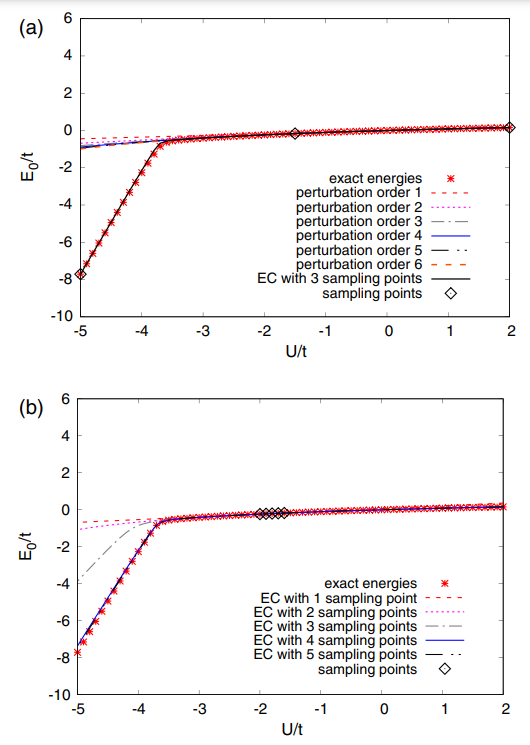
\includegraphics[width=0.8\linewidth]{./pt_vs_ec.png}
  \caption{Results for \ac{EC} applied to the three-dimensional Bose-Hubbard
  model on a 4 × 4 × 4 periodic lattice, reproduced from \cite{frame2018eigenvector}. The horizontal axis is $\lambda$, in this case a dimensionless coupling parameter. The vertical axis is the dimensionless ground state energy of the system. (a) and (b) differ by choice of subspace. Notably, in (b) although the training subspace (diamonds) is confined to a single phase of the system, \ac{EC} extrapolates the energy through the phase change with much greater accuracy than
  h
perturbation theory. }%
  \label{fig:pt_vs_ec}
\end{figure}
\section{\label{sec:lim} Selected results from literature}

In this section we reproduce and briefly discuss several interesting results from the literature, to give a survey of the applications listed in the first section.

In Fig. \ref{fig:exc}, reproduced from \cite{eklind2021eigenvector}, we see \ac{EC} applied to an ultra-cold 2-body system. Notice that 5 different energy levels are accurately reproduced, with a training subspace spanning only 2 of them. The interested reader is referred to this work for a discussion of optimal training subspace selection, and extension to excited states.

\begin{figure}[htpb]
  \centering
  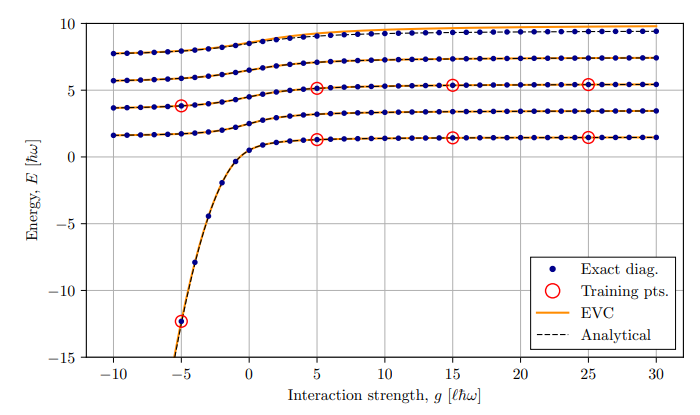
\includegraphics[width=0.99\linewidth]{./EC_vs_anal_excited.png}
  \caption{Prediction of energies of the ground and first 4 excited states of an ultra-cold 2-body system with harmonic interaction potential, as a function of the interaction strength, reproduced from \cite{eklind2021eigenvector}. Numerical and analytical solutions are compared to \ac{EC} solutions, with training subspace shown circled. Notice that the training subspace only samples from 2 levels, but accurately reconstructs all 5.}%
  \label{fig:exc}
\end{figure}

Several studies have highlighted the power of \ac{EC} as an emulator to make Bayesian studies computationally tractable. Most prominently, this has been applied to \ac{CEFT} nuclear structure calculations. Fig. \ref{fig:sense}, reproduced from \cite{ekstrom2019global}, shows the sensitivities of bulk nuclear properties of $^{16}$O, to the \ac{CEFT} \ac{LEC}s, calculated using a Bayesian global sensitivity analysis approach.  The sensitivity results are important to constrain LEC values, understand uncertainties, and focus  future experimental and theoretical work on the most sensitive observables and most
important LECs. 

Fig. \ref{fig:cov}, reproduced from \cite{konig2020eigenvector}, shows the covariance of bulk ground-state observables in the few-nucleon sector (ground state energies and charge raddi of $^2$H, $^3$H and $^4$He). Without \ac{EC}, this would likely be computationally intractable, but with the trained EC, the Bayesian analysis runs in minutes on an ordinary laptop. Teasing covariances out of complex models highlights correlations between observables, providing
vital conceptual feedback. It is worth noting that the \ac{UQ} done in both of these works is on experimentally measurable observables.

\begin{figure}[tpb]
  \centering
  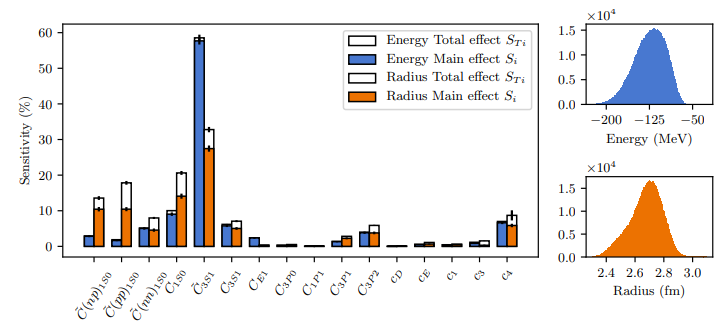
\includegraphics[width=0.99\linewidth]{./LEC_sensitivity.png}
  \caption{Sensitivity of bulk properties of the $^{16}$O nucleus, calculated with \ac{CEFT}, to the \ac{LEC}s, reproduced from \cite{ekstrom2019global}. Left bar for each \ac{LEC} is the sensitivity to ground state energy, right bar to charge radius. The horizontal axis groups the sensitivities by LEC. The panels on the right show the total uncertainty in ground state energy and charge radius.}
  \label{fig:sense}
\end{figure}


\begin{figure}[b]
  \centering
  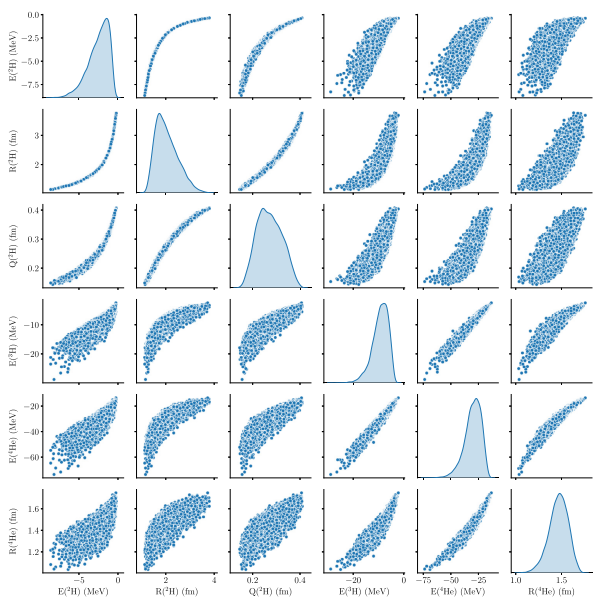
\includegraphics[width=1.0\linewidth]{./LEC_covar.png}
  \caption{Emulated sample of how selected observables in $^2$H, $^3$H, and $^4$ He co-vary with each other at 104 different values of the 16 LECs.}
\label{fig:cov}
\end{figure}


\section{\label{sec:appl} Conclusions}

We have reviewed the technique of \ac{EC}, which has enjoyed interest in the quantum mechanics literature over the last four years as a novel approximation technique. This technique has been used as an emulator for calculating eigenstates, energy levels, and scattering phase shifts in computationally expensive and non-perturbative systems. The convergence properties have been studied, and, in typical cases, are an improvement when compared to perturbative approaches.

It is the opinion of the author that this technique is underutilized, especially in the former approach; using it as an emulator for rapid Bayesian inference. The field of \ac{UQ} in theoretical physics is new but burgeoning, while the field of statistical Bayesian inference is mature and replete with robust algorithms for globally optimizing complex models over high-dimensional parameter spaces, to noisy data, with \ac{UQ}.
Often, when Bayesian approaches are applied to \ac{UQ}, computational constraints limit one to using to dimensionally-reduced surrogate models of the full model in question, with limited accuracy. \ac{EC} allows for a systematic, data-driven way to do construct these surrogate models, that is highly accurate as long the training subspace used is of high quality, and spans the space the parameters are extrapolated to. 

Additionally, one can't help but speculate about the effect of taking \ac{EC} to higher orders, e.g. including correction terms $\vec{c}^T \mathbf{H} \vec{c} \vec{c}^T \mathbf{H} \vec{c}$ and so on. This is pure speculation, as the analytical interpretation of this isn't immediately clear, but could be interesting to explore.

\bibliographystyle{plain}
\bibliography{apssamp}% Produces the bibliography via BibTeX.
\end{document}
%
% ****** End of file apssamp.tex ******
